\documentclass[11pt,a4paper]{article}

\usepackage[margin=2.3cm]{geometry}
\usepackage[T1]{fontenc}
\usepackage{lmodern}
\usepackage{microtype}
\usepackage{amsmath,amssymb}
\usepackage{booktabs}
\usepackage{tabularx}
\usepackage{enumitem}
\usepackage{xcolor}
\usepackage{tikz}
\usetikzlibrary{arrows.meta,positioning,fit,backgrounds}
\usepackage[hidelinks]{hyperref}
\usepackage{listings}

\definecolor{accent}{HTML}{1F4E79}
\definecolor{soft}{HTML}{E8EEF5}
\definecolor{warn}{HTML}{FFF4E0}
\definecolor{good}{HTML}{E6F4EA}

\lstset{basicstyle=\ttfamily\small,columns=fullflexible,frame=none,xleftmargin=1em}
\setlist{itemsep=2pt,topsep=4pt}
\newcommand{\code}[1]{\texttt{\small #1}}
\newcommand{\verdict}[2]{\noindent\colorbox{#1}{\parbox{\dimexpr\linewidth-2\fboxsep}{\small #2}}\par\medskip}

\title{\textbf{SLM Policy with Write-Sparse Spatio-Temporal Memory}\\[2pt]
\large Architecture, feasibility assessment, and reference implementation}
\author{SC4001 Group Project --- design note}
\date{4 November 2026}

\begin{document}
\maketitle

\begin{abstract}
\noindent This note evaluates the planned main model of the project: a small language model (SLM) that acts in the
BabyAI-Text gridworld, trained first by behaviour cloning and then by reinforcement learning (RL), with a GRU-like
component that controls a fixed-size memory of past views. We formalise the architecture, assess whether it can be
trained on the available hardware and before the deadline, and argue that a standard GRU is the wrong tool for a memory
whose content \emph{is} its output and should rarely change. We replace it with a \emph{write-sparse slot memory}: a
GRU whose update gate is factorised into a scalar ``save?'' gate and a slot address, with an identity path when nothing
is written. A reference implementation (\code{models/slm\_policy}, \code{training/}) with 16 tests accompanies the note.
\textbf{Verdict:} the architecture is feasible to build and to train on a single GPU, \emph{if} the SLM is kept out of
the recurrent path and the thinking mode is dropped from training. The main risk is scientific rather than
computational: in this environment the SLM and the memory may add little over a small non-language model, so the
ablations must be planned to show this either way.
\end{abstract}

\tableofcontents
\bigskip

%=====================================================================================
\section{Summary of findings}
%=====================================================================================

\begin{center}
\small
\begin{tabularx}{\linewidth}{@{}>{\raggedright\arraybackslash}p{3.6cm}>{\raggedright\arraybackslash}p{2.0cm}X@{}}
\toprule
Question & Verdict & Reason \\
\midrule
Can the model be built? & \textbf{Yes} & Implemented and tested end to end (\S\ref{sec:code}); a tiny random Qwen3 stands in for the SLM in tests. \\
Can an SLM be trained with RL like GLAM? & \textbf{Yes, for the easy tier} & One SLM forward per decision ($\approx$25 tokens), top layers frozen, LoRA on the bottom ones, behaviour-cloning warm start. Estimated 1--3\,GPU-hours per PPO run on an RTX~4060 class GPU (\S\ref{sec:compute}). Hard tier uncertain. \\
Is a GRU right for the memory? & \textbf{No, modify it} & A GRU rewrites its whole state every step and has a single-vector bottleneck. Use a write-sparse slot memory (\S\ref{sec:memory}). \\
SLM ``thinking'' mode in training? & \textbf{No} & Hundreds of generated tokens per step, up to 128 steps per episode, and no reasoning traces to imitate. Evaluate it zero-shot only, if at all. \\
Will the SLM help? & \textbf{Uncertain} & The mission vocabulary has 15 words; a word GRU learns it from demonstrations. The SLM's prior matters mostly on shifted test sets, and \code{test\_nonce} renames only the mission text (\S\ref{sec:risks}). \\
Will the memory help? & \textbf{Uncertain} & A 7$\times$7 view covers most of a 6$\times$6 room and expert episodes take 6--12 steps, so partial observability is mild. Plan a smaller-view variant (\S\ref{sec:recs}). \\
\bottomrule
\end{tabularx}
\end{center}

%=====================================================================================
\section{Architecture}
\label{sec:arch}
%=====================================================================================

At each environment step $t$ the policy receives the egocentric symbolic view $o_t \in \{0..10\}^{7\times7\times3}$, the
heading $\delta_t \in \{0,1,2,3\}$, the step index $t$ and the mission string $m$. It outputs a distribution over six
actions and a value estimate. Figure~\ref{fig:arch} shows the data flow.

\begin{figure}[ht]
\centering
\resizebox{\linewidth}{!}{%
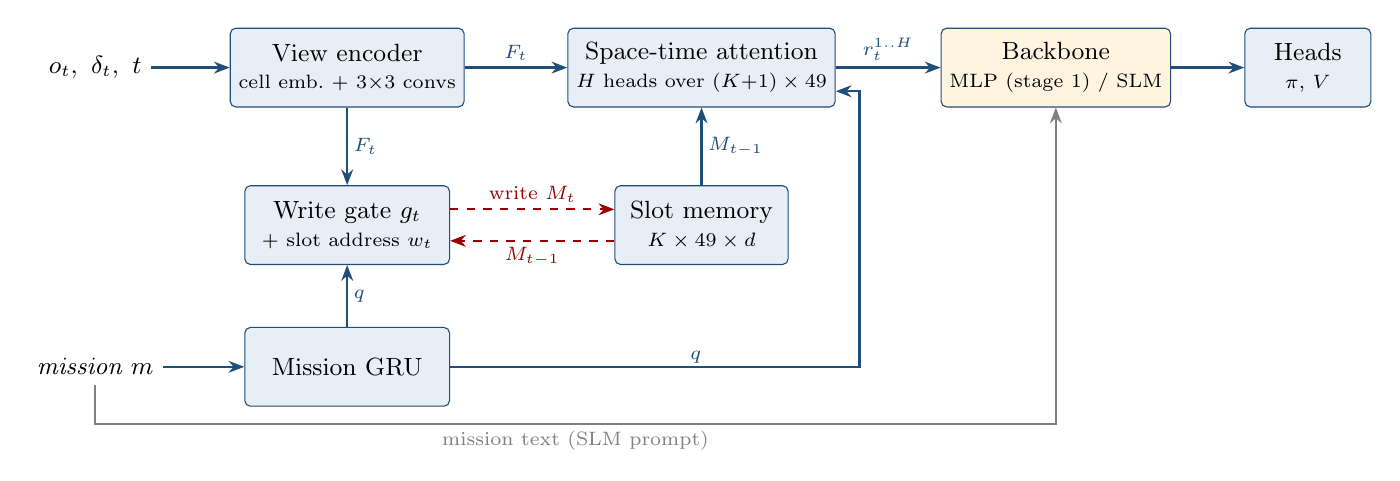
\begin{tikzpicture}[
  box/.style={draw=accent, fill=soft, rounded corners=2pt, minimum height=10mm, minimum width=26mm, align=center, font=\small, inner sep=3pt},
  slm/.style={box, fill=warn},
  io/.style={font=\small\itshape, align=center},
  arr/.style={-{Stealth[length=2mm]}, thick, accent},
  rec/.style={-{Stealth[length=2mm]}, thick, dashed, red!60!black},
  lab/.style={font=\scriptsize, fill=white, inner sep=1pt}]
  % row 1: the decision path
  \node[io]  (obs)   at (0,0)     {$o_t,\ \delta_t,\ t$};
  \node[box] (enc)   at (3.2,0)   {View encoder\\[-1pt]\scriptsize cell emb.\ + 3$\times$3 convs};
  \node[box, minimum width=30mm] (att) at (7.7,0) {Space-time attention\\[-1pt]\scriptsize $H$ heads over $(K{+}1)\times49$};
  \node[slm] (bb)    at (12.2,0)   {Backbone\\[-1pt]\scriptsize MLP (stage 1) / SLM};
  \node[box, minimum width=16mm] (heads) at (15.4,0) {Heads\\[-1pt]\scriptsize $\pi$, $V$};
  % row 2: the memory loop
  \node[box] (gate)  at (3.2,-2.0) {Write gate $g_t$\\[-1pt]\scriptsize + slot address $w_t$};
  \node[box, minimum width=22mm] (mem) at (7.7,-2.0) {Slot memory\\[-1pt]\scriptsize $K\times49\times d$};
  % row 3: the mission
  \node[io]  (mis)   at (0,-3.8)  {mission $m$};
  \node[box] (menc)  at (3.2,-3.8) {Mission GRU};

  \draw[arr] (obs) -- (enc);
  \draw[arr] (enc) -- node[lab, above=1pt]{$F_t$} (att);
  \draw[arr] (att) -- node[lab, above=1pt]{$r^{1..H}_t$} (bb);
  \draw[arr] (bb) -- (heads);
  \draw[arr] (enc) -- node[lab, right=1pt]{$F_t$} (gate);
  \draw[arr] (mem) -- node[lab, right=1pt]{$M_{t-1}$} (att);
  \draw[rec] ([yshift=2mm]gate.east) -- node[lab, above=1pt]{write $M_t$} ([yshift=2mm]mem.west);
  \draw[rec] ([yshift=-2mm]mem.west) -- node[lab, below=1pt]{$M_{t-1}$} ([yshift=-2mm]gate.east);
  \draw[arr] (mis) -- (menc);
  \draw[arr] (menc) -- node[lab, right=1pt]{$q$} (gate);
  \draw[arr] (menc.east) -- ++(5.2,0) node[lab, above, pos=0.6]{$q$} |- ([yshift=-3mm]att.east) ;
  \draw[arr, gray] (mis.south) -- ++(0,-0.5) -| node[lab, pos=0.25, below=1pt]{mission text (SLM prompt)} (bb.south);
\end{tikzpicture}}
\caption{Data flow for one step. The only recurrence (dashed) is the memory write, which never passes through the SLM.
The SLM (shaded) reads the mission as text and the $H$ read-outs as soft tokens.}
\label{fig:arch}
\end{figure}

\paragraph{View encoder.} Each cell's (object, colour, state) codes are embedded and summed with a learned
position embedding (the view is egocentric, so positions are meaningful), then mixed by residual $3\times3$
convolutions. Heading and a time encoding $e(t)$ are added:
$F_t = \mathrm{LN}\big(\mathrm{Conv}(E(o_t)) + P + E_\delta(\delta_t) + e(t)\big) \in \mathbb{R}^{49\times d}$.
$e(\cdot)$ is a learned linear map of sinusoidal features, so it also accepts fractional ages.

\paragraph{Mission encoder.} A word GRU gives $q \in \mathbb{R}^{d_q}$. It is deliberately \emph{separate from the
SLM}: the memory gate and the attention scorer need the mission at every step, and keeping the SLM out of the recurrent
path is what makes training affordable (\S\ref{sec:compute}).

\paragraph{Space-time attention.} The current view and the $K$ slots form the grid
$S_t = [F_t; M_{t-1}] \in \mathbb{R}^{(K+1)\times 49\times d}$, with the age encoding of each slot added. A
convolutional scorer shared over slots and conditioned on $q$ by FiLM~\cite{perez2018film} gives, per head $h$, the
two-dimensional space-time weight matrix
\begin{equation}
A^h_t = \operatorname{softmax}_{(\tau,p)}\big(s^h(S_t, q)_{\tau,p} + \log \phi_\tau\big) \in \Delta^{(K+1)\times 49},
\qquad r^h_t = \textstyle\sum_{\tau,p} A^h_t[\tau,p]\, W_v S_t[\tau,p],
\end{equation}
where $\phi_\tau \in [0,1]$ is the fill level of slot $\tau$ ($\phi_0 = 1$ for the current view), so slots never
written receive no weight. $A^h_t$ is returned for visualisation; it is the ``space-time weight matrix'' of the design
brief, computed per step rather than stored as one static matrix, which could not follow where the goal is.

\paragraph{Backbone.} Stage~1 uses a small MLP on $[r^1..r^H, q]$ (model M1). From stage~2 the SLM reads
\begin{center}
\code{Goal: <mission>\textbackslash nWhat you see and remember: <soft$_1$>…<soft$_H$>\textbackslash nNext action:}
\end{center}
where $\text{soft}_h = \mathrm{LN}(W_a r^h)$ is scaled to the SLM's embedding statistics. The feature is the hidden
state of the last token at layer $L_r$ (\code{readout\_layer}); layers above $L_r$ are removed, so reading from an
intermediate layer (proposal H2) is also cheaper. LoRA~\cite{hu2022lora} adapters (rank 8, $q$/$v$ projections) are
placed on layers $0..9$ from the start; their zero initialisation leaves the SLM unchanged until stage~3 trains them.

\paragraph{Heads.} $\pi(a\mid\cdot) = \operatorname{softmax}(W_\pi\,\mathrm{LN}(z))$ and $V = w_V^\top \mathrm{LN}(z)$.

\paragraph{Sizes.} With the defaults in \code{config.SLM} ($d{=}64$, $K{=}8$, $H{=}4$) everything except the SLM has
0.41\,M parameters. On Qwen3-0.6B~\cite{qwen3} (28 layers, width 1024), the trainable SLM-side parameters are the adapter
($\approx$68\,k), LoRA ($\approx$0.41\,M for 10 layers) and the heads.

%=====================================================================================
\section{The memory: why not a plain GRU}
\label{sec:memory}
%=====================================================================================

\subsection{What a GRU does}

A GRU~\cite{cho2014gru} updates its state, which is also its output, at every step:
\begin{align}
z_t &= \sigma(W_z x_t + U_z h_{t-1} + b_z), \qquad
\rho_t = \sigma(W_\rho x_t + U_\rho h_{t-1} + b_\rho), \\
\tilde h_t &= \tanh\big(W_h x_t + U_h(\rho_t \odot h_{t-1}) + b_h\big), \qquad
h_t = (1-z_t)\odot h_{t-1} + z_t \odot \tilde h_t .
\end{align}
The observation that \emph{``the output is the memory and it rarely needs to be updated''} is correct, and it exposes
three mismatches with what the design brief asks for:
\begin{enumerate}
  \item \textbf{Dense rewriting.} Nothing forces $z_t$ to be 0; trained update gates typically stay in the middle of
  their range, so the state is partially overwritten at every step and old content decays roughly as
  $\prod_k(1-z_k)$. ``Save this view or not'' is never an explicit decision.
  \item \textbf{One-vector bottleneck.} All of the past must fit into one vector $h_t$. The spatial structure of the
  views (which cell held what) is lost, so the attention cannot point at \emph{where} in a past view something was.
  \item \textbf{The candidate mixes.} $\tilde h_t$ is a nonlinear blend of the new input and the old state, so even a
  write changes what was stored rather than storing the observation.
\end{enumerate}

\subsection{Write-sparse slot memory (implemented)}

We keep the GRU's interpolation form but change the gate, the candidate and the state:
\begin{align}
g_t &= \sigma\big(w_g^\top[\bar F_t,\ \bar M_{t-1},\ q,\ e(t)] + b_g\big) \in (0,1)
  && \text{``is this view worth saving?''} \\
w_t &= \operatorname{softmax}_k\big(a([\bar F_t,\ \bar M_{t-1}[k],\ \log(1+\alpha_k),\ \phi_k])\big) \in \Delta^K
  && \text{``which slot does it replace?''}\\
M_t[k] &= (1 - g_t w_t[k])\, M_{t-1}[k] + g_t w_t[k]\, F_t \\
\alpha_k &\leftarrow 1 + (1-g_t w_t[k])\,\alpha_k, \qquad \phi_k \leftarrow \phi_k + g_t w_t[k](1-\phi_k)
  && \text{age and fill of each slot}
\end{align}
Bars denote means over cells (and over filled slots for $\bar M$). Compared with a GRU:
\begin{itemize}
  \item the vector update gate $z_t$ is factorised into a scalar \emph{whether} ($g_t$) and a slot \emph{where}
  ($w_t$), as in the write heads of the NTM and DNC~\cite{graves2014ntm,graves2016dnc};
  \item the candidate is the encoded view $F_t$ itself, so a slot holds an actual (soft) past observation;
  \item there is no reset gate, because the current view is always read next to the memory: the memory only has to
  hold what is no longer visible, which is exactly why writes should be rare;
  \item when $g_t = 0$, $M_t = M_{t-1}$ and $\partial M_t / \partial M_{t-1} = I$: content does not decay between
  writes, and gradients through long gaps neither vanish nor explode.
\end{itemize}

\subsection{Making writes rare}

Four mechanisms, all in the code and configurable:
\begin{enumerate}
  \item \textbf{Bias initialisation.} $b_g = -2$ ($g \approx 0.12$), so ``do not write'' is the default, in the spirit
  of chrono-initialisation of gated RNNs~\cite{tallec2018chrono}.
  \item \textbf{Write penalty.} $\lambda_w\, \overline{g_t}$ is added to both the BC and the PPO loss
  (\code{BC.write\_penalty}, \code{PPO.write\_penalty}).
  \item \textbf{Hard gates.} \code{write\_mode="hard"} uses $\mathbb{1}[g_t > 0.5]$ in the forward pass and the
  straight-through gradient~\cite{bengio2013st} in the backward pass, as in Skip~RNN~\cite{campos2018skiprnn}; the
  memory is then bit-for-bit unchanged on non-writing steps (tested). Train soft first, switch to hard later.
  \item \textbf{Time conditioning.} $e(t)$ is an input to the gate, so the model can learn to store more early in an
  episode. If ``more picky as training progresses'' (open question~2 of the models README) is meant over \emph{training},
  increase $\lambda_w$ on a schedule; the per-step time input alone cannot do that.
\end{enumerate}
\textbf{Failure mode to monitor:} with short demonstrations that never need memory, the penalty can drive $g_t \to 0$
everywhere (``gate collapse''). The trainers log \code{write\_rate}; if it collapses, start with $\lambda_w = 0$.

\subsection{Alternatives considered}

\begin{center}
\small
\begin{tabularx}{\linewidth}{@{}>{\raggedright\arraybackslash}p{3.6cm}X@{}}
\toprule
Design & Assessment \\
\midrule
Plain GRU / LSTM~\cite{hochreiter1997lstm} & Simplest; the B3 baseline already covers ``no structured memory''. Problems listed above. \\
Transformer over all past views~\cite{parisotto2020gtrxl} & No write decision at all; cost grows with episode length. A useful upper-bound ablation, not the brief's design. \\
NTM / DNC~\cite{graves2014ntm,graves2016dnc} & Content-addressed reads and writes with usage tracking; more machinery than needed for $K{=}8$ slots. Our memory is a stripped-down version. \\
Allocentric map~\cite{parisotto2018neuralmap} & Writes each seen cell into a room-aligned map, solving the egocentric-frame problem (\S\ref{sec:risks}); needs the agent's position, which \code{babytext} does not expose in \code{info}. Strong future option. \\
\bottomrule
\end{tabularx}
\end{center}

%=====================================================================================
\section{Feasibility of RL with the SLM in the loop}
\label{sec:compute}
%=====================================================================================

\subsection{What makes it affordable}

GLAM~\cite{carta2023glam} fine-tuned all of Flan-T5 with PPO and scored the six action strings at every step, on a
multi-GPU setup. The present design is much cheaper per decision:
\begin{enumerate}
  \item \textbf{One forward pass per decision.} An action head on one hidden state instead of scoring six strings or generating text.
  \item \textbf{Short, fixed input.} About 25 tokens (mission + $H{=}4$ soft tokens + suffix), whatever the episode length, instead of GLAM's growing prompt with 3 observations.
  \item \textbf{No SLM in the recurrence.} The memory update depends only on the encoder and the mission GRU. In a
  $(B,T)$ training block the cheap recurrent loop runs first, and the SLM then processes all $B\cdot T$ steps \emph{in
  one batch}. A test checks that this gives the same logits as stepping one step at a time, which PPO needs for correct
  importance ratios.
  \item \textbf{Frozen top, LoRA bottom.} Gradients still flow \emph{through} the frozen top layers to reach LoRA and
  the adapter, but no weight gradients are computed for them: the backward pass costs about one forward pass instead of two.
  \item \textbf{Gradient checkpointing} (on by default) keeps activation memory within a laptop GPU (below).
  \item \textbf{Optional truncation.} Reading at an intermediate layer $L_r$ removes the layers above it.
\end{enumerate}

\subsection{Compute estimate}

Qwen3-0.6B has about $0.44$\,B non-embedding parameters, so a forward pass costs about
$2 \times 0.44\text{\,B} \times 25 \approx 22$\,GFLOP per decision. With $E$ PPO epochs, each sample costs one rollout forward plus
$E \times (1\ \text{fwd} + 1\ \text{bwd} + 1\ \text{recompute})$:
\begin{equation}
C_{\text{PPO}} \approx (1 + 3E)\times 22\ \text{GFLOP} = 286\ \text{GFLOP per environment step}\quad (E=4).
\end{equation}
\begin{center}
\small
\begin{tabular}{@{}lrrr@{}}
\toprule
Workload & FLOP & @ 10 TFLOP/s & @ 30 TFLOP/s \\
\midrule
BC (stage 2/3): 24\,k demo steps $\times$ 20 epochs & $3.2\times10^{16}$ & 53 min & 18 min \\
PPO, 200\,k environment steps & $5.7\times10^{16}$ & 1.6 h & 0.5 h \\
PPO, 1\,M environment steps & $2.9\times10^{17}$ & 8 h & 2.7 h \\
\bottomrule
\end{tabular}
\end{center}
These are \emph{order-of-magnitude} figures. 10\,TFLOP/s is a cautious effective bf16 throughput for an RTX~4060 laptop
GPU with small, ragged batches; 30\,TFLOP/s is plausible on a desktop RTX~5080. Validation rollouts (single environment,
batch size 1) are latency-bound and add a few minutes per evaluation. Stage~1 needs no SLM and runs on a CPU (about a minute per epoch, \S\ref{sec:results}).

\paragraph{GPU memory.} Weights: 1.2\,GB (bf16). A PPO minibatch of 4 sequences $\times$ 128 steps $\times$ 25 tokens
is 12.8\,k tokens. With checkpointing, the stored layer inputs take $12.8\text{k} \times 1024 \times 2\,\text{B} \times 28 \approx 0.73$\,GB,
plus about 0.5\,GB for the one layer being recomputed. Without checkpointing it would be about 12\,GB, which does not fit
in 8\,GB. \code{PPO.minibatch\_envs} is the knob to turn if memory runs out.

\paragraph{Sample efficiency.} The easy tasks have a high random floor (0.32 on \code{goto}) and short expert
solutions, and the policy starts from behaviour cloning, so PPO mainly corrects compounding errors. We expect
$10^5$--$2\times10^5$ steps to be enough on the easy tier. The hard tier (2\,\% random success on \code{putnext}) is
where sparse rewards start to matter, and potential-based shaping~\cite{ng1999shaping} towards the current sub-goal is
included for it.

\subsection{Schedule}

From 4 to 16 November there are 12 days. The full matrix (M1--M4 $\times$ 3 seeds $\times$ 2 tiers, plus ablations)
would take roughly 40--60 GPU-hours at the cautious rate. This is achievable only if runs are started early and stage~4
is limited to one task tier; see \S\ref{sec:recs} for the priorities.

%=====================================================================================
\section{Risks and open problems}
\label{sec:risks}
%=====================================================================================

\begin{enumerate}
  \item \textbf{The SLM may add nothing measurable.} The mission vocabulary is 15 words, and the GRU sees all of them
  in training (held-out goals hold out \emph{combinations}, e.g.\ ``yellow box''; ``yellow'' and ``box'' still occur).
  On \code{test\_nonce} only the mission text is renamed, and neither the SLM nor the GRU can map ``dueno'' to the
  grid's ``red'' code. Expect M1 $\approx$ M2/M3 in distribution. This is a valid result if it is reported as such.
  \item \textbf{The memory may add nothing measurable.} The 7$\times$7 view covers most of the 6$\times$6 room, so the
  goal is usually visible; expert episodes take 6--12 steps. The $K{=}0$ ablation is likely to be close to the full model.
  \item \textbf{Egocentric slots.} A stored view is in the agent's frame at the time of writing; after the agent turns,
  cell $p$ of an old slot is a different place. Heading and age are given to the reader, but the alignment has to be
  learned. An allocentric map would remove the problem.
  \item \textbf{Thinking mode.} It cannot be learned by BC (no traces), and it is prohibitively slow inside the PPO
  loop. It is not implemented; at most, compare it zero-shot at evaluation time.
  \item \textbf{Value head on the SLM feature.} Value and policy share LoRA gradients. If PPO is unstable, detach the
  value head's input or give it its own small MLP on the read-outs.
  \item \textbf{Forgetting the BC policy during RL.} Not handled. A KL penalty towards the stage-3 policy is the
  standard fix, but it costs a second SLM forward pass per sample.
  \item \textbf{Shaping needs environment internals.} The potential reads \code{agent\_pos} and \code{carrying} from the
  MiniGrid level. This access is confined to \code{training/vec\_env.py}.
\end{enumerate}

%=====================================================================================
\section{Training}
\label{sec:training}
%=====================================================================================

\begin{center}
\small
\begin{tabularx}{\linewidth}{@{}cp{1.6cm}X@{}}
\toprule
Stage & Algorithm & Trained (lr scale) \hfill frozen: everything else \\
\midrule
1 & BC & encoder, mission, memory, attention, readout MLP, action head (all 1.0) \\
2 & BC & adapter, new action head (1.0); encoder, mission, memory, attention (0.1); SLM and LoRA frozen \\
3 & BC & stage 2 + LoRA on SLM layers 0--9 (1.0) \\
4 & PPO & stage 3 + value head (1.0) \\
\bottomrule
\end{tabularx}
\end{center}
The table is data (\code{training/stages.py}); \code{make\_optimizer} freezes every parameter outside a stage's groups.

\paragraph{Behaviour cloning.} Whole episodes in time order, padded and masked ($\mathcal{M}$ = real steps):
\begin{equation}
\mathcal{L}_{\text{BC}} = -\frac{1}{|\mathcal{M}|}\sum_{(b,t)\in\mathcal{M}} \log \pi(a^\ast_{b,t}\mid\cdot) + \lambda_w \bar g,
\end{equation}
with full back-propagation through time (episodes are short). After every epoch, the trainer computes the demo loss on
val demos and greedy success on val seeds, and keeps the best checkpoint.

\paragraph{Rewards.} Immediate:
\begin{equation}
r_t = r^{\text{env}}_t + \lambda_s\big(\gamma\,\Phi(s_{t+1}) - \Phi(s_t)\big), \qquad
\Phi(s) = -\frac{\text{dist}(\text{agent},\ \text{nearest current goal object})}{\text{room size}},
\end{equation}
where the current goal is the second named object once the first is carried, and $\Phi = 0$ at terminal
states, so the optimal policy is unchanged~\cite{ng1999shaping}. Delayed: the discounted return, estimated by GAE~\cite{schulman2016gae}:
\begin{equation}
\hat A_t = \sum_{l\ge0} (\gamma\lambda)^l \delta_{t+l}, \qquad \delta_t = r_t + \gamma V(s_{t+1})(1-d_t) - V(s_t).
\end{equation}

\paragraph{Recurrent PPO.} $N$ environments $\times$ $T$ steps. Each environment's rollout is one sequence; the memory at
its start is stored (as in R2D2~\cite{kapturowski2019r2d2}), and episode boundaries inside it reset the memory. Each
minibatch replays whole sequences, so the delayed reward trains the gate and the attention through time:
\begin{equation}
\mathcal{L} = -\mathbb{E}\big[\min(\rho_t \hat A_t,\ \operatorname{clip}(\rho_t, 1\pm\epsilon)\hat A_t)\big]
+ c_V\,\mathbb{E}[(V - \hat R)^2] - c_H\,\mathbb{E}[\mathcal{H}(\pi)] + \lambda_w \bar g
\end{equation}
\cite{schulman2017ppo}. The defaults in \code{config.PPO} are $N{=}16$, $T{=}128$, 4 epochs, 4 sequences per minibatch,
$\epsilon{=}0.2$ and $\lambda_s{=}0.1$.

%=====================================================================================
\section{Reference implementation}
\label{sec:code}
%=====================================================================================

\begin{lstlisting}
config.py                SLM, BC, PPO sections (all tunable values)
models/slm_policy/       the model; imports babytext + config, never training
  inputs.py              Observations (B,T) block; observations_from_env; MissionTable
  encoders.py            TimeEncoding, ViewEncoder, MissionEncoder
  memory.py              MemoryState, SlotMemory (write-sparse "modified GRU")
  attention.py           SpaceTimeAttention -> read-outs + (K+1)x49 weight matrix
  backbones.py           Backbone interface; ReadoutBackbone; SLMBackbone (LoRA, truncation)
  policy.py              SLMPolicy, PolicyOutput, parameter_groups, save/load_model
  agent.py               SLMAgentPolicy: a babytext policy (obs -> action)
training/
  vec_env.py             ALL environment plumbing for RL: autoreset, seeds, t, shaping potential
  rewards.py             shaped_reward, compute_gae (pure maths)
  demos.py               demo files -> padded (B,T) batches
  stages.py              the stage table + make_optimizer (freezing)
  bc.py / ppo.py         the two trainers
  train.py               CLI: python -m training.train --stage N ...
tests/test_slm_policy.py 16 tests (tiny random Qwen3, CPU, ~7 s)
\end{lstlisting}

\paragraph{Design principles.}
\begin{itemize}
  \item \textbf{The environment is separate.} \code{babytext} is unchanged. Everything RL needs from the environment
  (vectorising, automatic resets on the correct seed split, step counters, the private \code{agent\_pos}) is in one
  adapter, \code{training/vec\_env.py}, so PPO only sees arrays.
  \item \textbf{One code path for acting and learning.} \code{SLMPolicy.forward} takes a $(B,T)$ block; acting is
  $T{=}1$. Rollout and update therefore cannot drift apart (this is tested).
  \item \textbf{Swappable backbone (strategy pattern).} The model reaches the backbone only through
  \code{Backbone.forward}, so M1, the SLM, another SLM or a different prompt are local changes.
  \item \textbf{Stages and settings are data.} The stage table and the \code{config} dataclasses hold every choice; the
  trainers contain no stage-specific branches.
  \item \textbf{Dependencies point one way:} \code{babytext} $\leftarrow$ \code{models} $\leftarrow$ \code{training}.
  Checkpoints exclude the frozen SLM weights, so a trained model loads without the training code.
  \item \textbf{Documented public API.} Each package lists its public names in \code{\_\_all\_\_} and its module
  docstring. Public functions document their arguments and tensor shapes.
\end{itemize}

\paragraph{Usage.}
\begin{lstlisting}
python -m training.tools.collect_demos
python -m training.train --stage 1 --tasks goto pickup --out outputs/runs/m1
python -m training.train --stage 2 --init outputs/runs/m1/best.pt --out outputs/runs/m2
python -m training.train --stage 3 --init outputs/runs/m2/best.pt --out outputs/runs/m3
python -m training.train --stage 4 --init outputs/runs/m3/best.pt --out outputs/runs/m4
\end{lstlisting}
Stages 2--4 need \code{pip install -e ".[models]"} plus \code{peft}.

\paragraph{Why not torch-ac / rl-starter-files?} The \code{rl-starter-files} repository and its PPO library
\code{torch-ac} are a proven baseline for MiniGrid. We read them before deciding against using them as a dependency:
\begin{itemize}
\item They cover only stage~4; stages~1--3 still need our own code.
\item Their recurrent interface expects a flat memory vector stored at every frame.
\item Their \code{ParallelEnv} resets environments without seeds, which would mix our train, val and test layouts.
\item They call \code{multiprocessing.set\_start\_method("fork")} at import, which fails on Windows.
\item They use a single learning rate for all parameters.
\end{itemize}
Our PPO module is about 200 lines and follows the same algorithm.

%=====================================================================================
\section{Initial results}
\label{sec:results}
%=====================================================================================

These checks show that the pipeline works and how expensive it is. They are \emph{not} tuned results: they used
500 demonstrations per task (a quarter of \code{config.DATA}), a CPU only, and a single seed.

\paragraph{Integration with the real SLM.} \code{SLMBackbone} was loaded with \code{Qwen/Qwen3-0.6B} and run forward
and backward through stage~3's optimiser on 8 steps. The prompt is 22 tokens long (with the 4 soft tokens), close to the
25 assumed in \S\ref{sec:compute}. The trainable groups are: encoder 117.7\,k, mission GRU 62.8\,k, memory gate 8.8\,k,
attention 57.9\,k, adapter 68.6\,k, LoRA 409.6\,k, action head 8.2\,k and value head 1.0\,k parameters. LoRA receives
non-zero gradients and none of the frozen SLM weights receive any.

\paragraph{Stage 1 (no SLM).}
\begin{center}
\small
\begin{tabularx}{\linewidth}{@{}Xccccc@{}}
\toprule
Run & Updates & Val CE & Val acc. & Write rate & Val success \\
\midrule
A: goto + pickup, lr $3\times10^{-4}$, batch 32, 12 epochs & 375 & 0.81 & 0.66 & 0.13 & 0.30 / 0.12 \\
B: goto only, lr $10^{-3}$, batch 8, 25 epochs & 1\,575 & 0.67 & 0.73 & 0.09 $\to$ 0.04 & 0.50 \\
\midrule
Random policy & -- & -- & -- & -- & 0.31 / 0.13 \\
\bottomrule
\end{tabularx}\\[2pt]
\footnotesize Val CE is the best epoch; val success is greedy, goto / pickup, after the last epoch (100 episodes per task for A, 200 for B).
\end{center}
Observations:
\begin{itemize}
  \item \textbf{The defaults train too slowly.} With \code{config.BC} defaults and 500 demonstrations per task, an
  epoch is only $\approx$31 updates, and after 12 epochs the policy is still at the random floor.
  \item \textbf{The model can fit the data, but overfits a small demo set.} With more updates the training
  cross-entropy falls to 0.10 while the validation cross-entropy rises after epoch~9. The final greedy success on goto
  is 0.50 (200 val episodes), well above the random 0.31 but far from the expert's 1.0. Use all 2\,000 demonstrations
  per task, select checkpoints on val, and consider DAgger.
  \item \textbf{The gate starts to collapse.} The write rate drops from 0.09 to 0.04 as training goes on. This is the
  failure mode described in \S\ref{sec:memory}: these demonstrations reward little memory, so the penalty and the
  negative bias win. Run one stage-1 variant with \code{write\_penalty = 0}.
  \item \textbf{Timing.} Stage~1 takes about 1 minute per epoch on a 22-core CPU, mostly spent in the 100-episode
  validation rollouts. Batched validation would speed this up considerably.
\end{itemize}


%=====================================================================================
\section{Recommendations}
\label{sec:recs}
%=====================================================================================

\begin{enumerate}
  \item \textbf{Run stage~1 now} (CPU is enough) on both tiers, 3 seeds, with all 2\,000 demonstrations per task and
  more updates than the current \code{config.BC} defaults give (\S\ref{sec:results}). M1 versus B3 already answers ``does the learned
  memory beat a fixed window?''.
  \item \textbf{Stages 2--3 on the easy tier first}, with the read-out layer as the only sweep (e.g.\ 10, 18, 28). This
  keeps the proposal's layer question (H2) alive and makes the cheaper settings faster.
  \item \textbf{Stage~4 on one configuration}, easy tier, 200\,k steps, 3 seeds. Extend to the hard tier only if time remains.
  \item \textbf{Make memory necessary in one experiment.} For example, reduce \code{ENV.agent\_view\_size} to 3 or 5,
  or evaluate on \code{test\_dist16}. Otherwise the $K{=}0$ ablation will probably show no difference, and the reason
  will be the environment, not the memory.
  \item \textbf{Drop the thinking mode from training}; mention it as future work.
  \item \textbf{Report the write rate and space-time attention maps.} \code{SLMAgentPolicy} records them when
  created with \code{keep\_attention=True}. They are inexpensive and make the memory's behaviour visible in the report.
\end{enumerate}

%=====================================================================================
\begin{thebibliography}{99}\small
\bibitem{bengio2013st} Y.~Bengio, N.~L\'eonard, A.~Courville. Estimating or propagating gradients through stochastic neurons for conditional computation. \emph{arXiv:1308.3432}, 2013.
\bibitem{campos2018skiprnn} V.~Campos, B.~Jou, X.~Gir\'o-i-Nieto, J.~Torres, S.-F.~Chang. Skip RNN: Learning to skip state updates in recurrent neural networks. \emph{ICLR}, 2018.
\bibitem{carta2023glam} T.~Carta, C.~Romac, T.~Wolf, S.~Lamprier, O.~Sigaud, P.-Y.~Oudeyer. Grounding large language models in interactive environments with online reinforcement learning. \emph{ICML}, 2023.
\bibitem{cho2014gru} K.~Cho et al. Learning phrase representations using RNN encoder--decoder for statistical machine translation. \emph{EMNLP}, 2014.
\bibitem{graves2014ntm} A.~Graves, G.~Wayne, I.~Danihelka. Neural Turing machines. \emph{arXiv:1410.5401}, 2014.
\bibitem{graves2016dnc} A.~Graves et al. Hybrid computing using a neural network with dynamic external memory. \emph{Nature} 538, 2016.
\bibitem{hochreiter1997lstm} S.~Hochreiter, J.~Schmidhuber. Long short-term memory. \emph{Neural Computation} 9(8), 1997.
\bibitem{hu2022lora} E.~J.~Hu et al. LoRA: Low-rank adaptation of large language models. \emph{ICLR}, 2022.
\bibitem{kapturowski2019r2d2} S.~Kapturowski, G.~Ostrovski, J.~Quan, R.~Munos, W.~Dabney. Recurrent experience replay in distributed reinforcement learning. \emph{ICLR}, 2019.
\bibitem{ng1999shaping} A.~Y.~Ng, D.~Harada, S.~Russell. Policy invariance under reward transformations: theory and application to reward shaping. \emph{ICML}, 1999.
\bibitem{parisotto2018neuralmap} E.~Parisotto, R.~Salakhutdinov. Neural Map: Structured memory for deep reinforcement learning. \emph{ICLR}, 2018.
\bibitem{parisotto2020gtrxl} E.~Parisotto et al. Stabilizing transformers for reinforcement learning. \emph{ICML}, 2020.
\bibitem{perez2018film} E.~Perez, F.~Strub, H.~de Vries, V.~Dumoulin, A.~Courville. FiLM: Visual reasoning with a general conditioning layer. \emph{AAAI}, 2018.
\bibitem{qwen3} Qwen Team. Qwen3 technical report. \emph{arXiv:2505.09388}, 2025.
\bibitem{schulman2016gae} J.~Schulman, P.~Moritz, S.~Levine, M.~Jordan, P.~Abbeel. High-dimensional continuous control using generalized advantage estimation. \emph{ICLR}, 2016.
\bibitem{schulman2017ppo} J.~Schulman, F.~Wolski, P.~Dhariwal, A.~Radford, O.~Klimov. Proximal policy optimization algorithms. \emph{arXiv:1707.06347}, 2017.
\bibitem{tallec2018chrono} C.~Tallec, Y.~Ollivier. Can recurrent neural networks warp time? \emph{ICLR}, 2018.
\end{thebibliography}

\end{document}
